\section{Anonymous ATXO transaction}



\begin{figure}[h]
	\caption{Example of a parametric plot ($\sin (x), \cos(x), x$)}
	\centering
	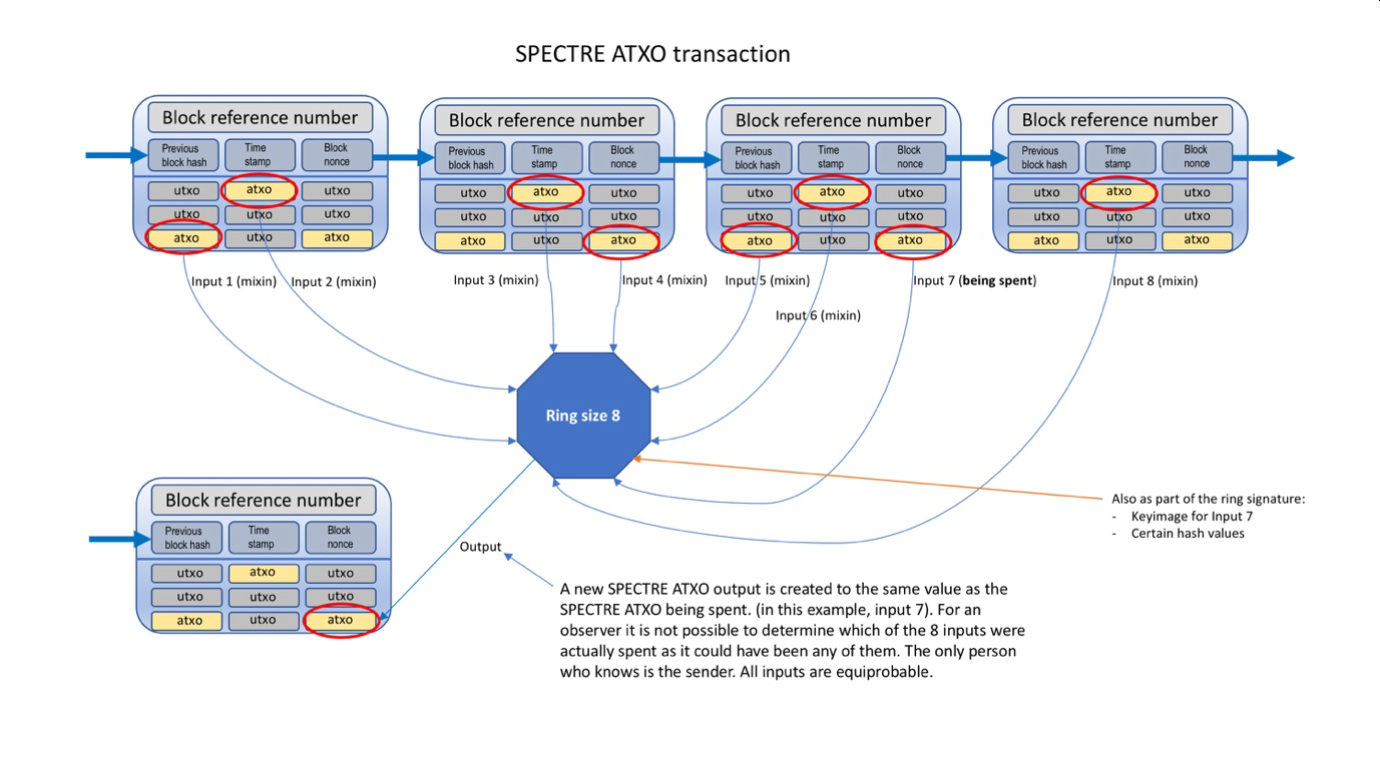
\includegraphics[width=\textwidth]{Anonymous-ATXO-Transaction.png}
\end{figure}



In the Spectrecoin software we talk about ring sizes and this refers to the
group or set of possible signers. So, in the example below, we have a ring
size of 8 which simply means that amongst the 8 public keys that form part
of the digital signature, 7 are so called ‘\textit{mixins}’ or chaff or decoys and
only 1 is the public key corresponding to the SPECTRE being spent. When
conducting an anonymous transaction, we use ring signatures to hide spent
output in a set of the same denomination.



Anonymous transactions in Spectrecoin can be said to have levels of
‘\textit{transactional entropy}’ as there is an interface between the ‘\textit{public}’
and the ‘\textit{anonymous}’ coins. Entropy level 0 can be said to be at the
interface between XSPEC >> SPECTRE and between SPECTRE >> XSPEC. Once
SPECTRE has been created from SPECTRE, i.e. an ATXO used as an input to
create a new ATXO we can say that this is entropy level 1 as the freshly
created ATXO has no public UTXO origin. Once these ATXOs are used to
create further ATXOs this would be entropy level 2 and so on. The entropy
increases with every level, IF AND ONLY IF a minimum ring size is used and
the ATXOs have not been part of any ring size 1 transaction.
